\documentclass{amsart}
\usepackage{amsfonts} % For math fonts
\usepackage{amsmath, amssymb, amsthm}
\usepackage{float}
\usepackage{enumitem}
\usepackage{graphicx}
\usepackage{listings} % For custom coding font
\usepackage{xcolor}

\lstset{
    language=Python,
    backgroundcolor=\color{gray}, % Light gray background
    basicstyle=\ttfamily\small\color{white}, % Code style
    keywordstyle=\color{cyan}\bfseries, % Keywords style
    stringstyle=\color{yellow}, % Strings style
    commentstyle=\color{black}, % Comments style
    frame=single, % Box around code
    rulecolor=\color{white}, % Frame color
    numbers=left, % Line numbers
    numberstyle=\tiny\color{white}, % Line number style
    breaklines=true, % Automatic line breaking
    showstringspaces=false
}

\setlist[enumerate,1]{label=\arabic*.}
\setlist[enumerate,2]{label=\alph*.,itemindent=2em}
\setlist{topsep=0pt, leftmargin=*, labelsep=1em}

\title{HW5 CS 180}
\author{Asher Christian 006-150-286}
\date{ 24.02.25}

\begin{document}
\maketitle

\section{Exercise 1}
\emph{
    Given an unsorted integer array, find all pair with given difference k in it without using any
    extra space.
    arr = [1,5,2,2,2,5,5,4] k =3
    Output: (2,5) and (1,4)
}

\section{Exercise 3 P 314}
For part (a)
consider the graph with the nodes
$v_1,v_2,v_3,v_4,v_5$
with the edges
\[
    (v_1,v_2), (v_1,v_3), (v_2,v_5), (v_3,v_4), (v_4,v_5)
.\] 
\begin{figure}[H]
    \centering
    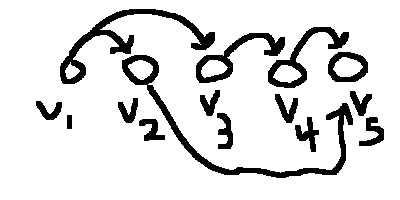
\includegraphics[width=0.8\textwidth]{example_graph.png}
\end{figure}
This algorithm would find the shortest path to be of length 2 since it greedily picks the node
with the least index. It would thus first pick the edge leading to vertex 2 and then from there the only edge possible is vertex 5.
If instead the edges $(v_1,v_3),(v_3,v_4),(v_4,v_5)$ were picked, the length would be 3.
\\
For part (b):\\
Let opt(i) be the length of the longest path to vertex $i$. For each vertex, if there are no incoming
edges then opt(i) = -inf, if there are incoming edges $opt(i) = 1 + \max_{k}\{opt(k)\}$ where $k \in \{\text{vertices with edges ending in vertex $i$}\}$. and
we set explicitely opt(0) = 0. If we compute opt(i) for each i, then opt(n) is the longest path to vertex n.
I prove the validity of this algorithm inductively.
Clearly for $v_1$ the longest path from $v_1$ to $v_1$ is zero since no edges can end on $v_1$ by the rule that every edge starts at 
a lower index than it ends at and no index is less than 1.
Inductively assume that we find the shortest path to all vertices up to $i-1$ then for vertex $i$, the longest path to vertex $i$ must pass
through an edge that goes into vertex $i$, all of those edges are ones that have been already discovered and found their longest paths by the inductive hypothesis
and thus the longest path to vertex $i$ is the longest path to a vertex that has an edge leading to vertex  $i$ plus one, which is exactly what $opt(i)$ computes. Thus $opt(i)$ is
the longest path to every vertex.
\\
The algorithm is as follows
\begin{lstlisting}
\end{lstlisting}


\end{document}
